\let\negmedspace\undefined
\let\negthickspace\undefined
\documentclass[journal]{IEEEtran}
\usepackage[a5paper, margin=10mm, onecolumn]{geometry}
%\usepackage{lmodern} % Ensure lmodern is loaded for pdflatex
\usepackage{tfrupee} % Include tfrupee package

\setlength{\headheight}{1cm} % Set the height of the header box
\setlength{\headsep}{0mm}     % Set the distance between the header box and the top of the text

\usepackage{gvv-book}
\usepackage{gvv}
\usepackage{cite}
\usepackage{amsmath,amssymb,amsfonts,amsthm}
\usepackage{algorithmic}
\usepackage{graphicx}
\usepackage{siunitx}
\usepackage{textcomp}
\usepackage{xcolor}
\usepackage{txfonts}
\usepackage{listings}
\usepackage{enumitem}
\usepackage{mathtools}
\usepackage{gensymb}
\usepackage{comment}
\usepackage[breaklinks=true]{hyperref}
\usepackage{tkz-euclide} 
\usepackage{listings}
% \usepackage{gvv}                                        
\def\inputGnumericTable{}                                 
\usepackage[latin1]{inputenc}                                
\usepackage{color}                                            
\usepackage{array}                                            
\usepackage{longtable}                                       
\usepackage{calc}                                             
\usepackage{multirow}                                         
\usepackage{hhline}                                           
\usepackage{ifthen}                                           
\usepackage{lscape}
\begin{document}

\bibliographystyle{IEEEtran}
\vspace{3cm}

\title{DIGITAL CLOCK}
\author{EE24BTECH11023 - RASAGNA}

% \maketitle
% \newpage
% \bigskip
{\let\newpage\relax\maketitle}

\renewcommand{\thefigure}{\theenumi}
\renewcommand{\thetable}{\theenumi}
\setlength{\intextsep}{10pt} % Space between text and floats


\numberwithin{equation}{enumi}
\numberwithin{figure}{enumi}
\renewcommand{\thetable}{\theenumi}

\section{Objective}
The objective of this project is to design and implement a digital clock using six common-anode seven-segment displays and an Arduino. The clock accurately displays hours, minutes, and seconds .The focus is on direct control of the displays using Arduino's digital I/O pins while implementing precise timekeeping through software-based delay function. This project demonstrates an understanding of seven-segment display interfacing and multiplexing techniques.

\section{Components and Equipment}

\begin{table}[h]
    \centering
    \renewcommand{\arraystretch}{1.2}
    \begin{tabular}{|c|l|c|}
        \hline
        \textbf{S.No} & \textbf{Component} & \textbf{Quantity} \\
        \hline
         1& Arduino  & 1 \\
         2& Breadboard & 1 \\
         3& Common-anode Seven segment displays & 6  \\
         4& USB A to USB B cable & 1 \\
         5& OTG adapter & 1 \\
         6& Jumper wires (Male-Male)& 70 \\
         7& Resistors \SI{220}{\ohm} & 6 \\
        \hline
    \end{tabular}
\end{table}

\section{Circuit Diagram and Schematic}

\begin{center}
    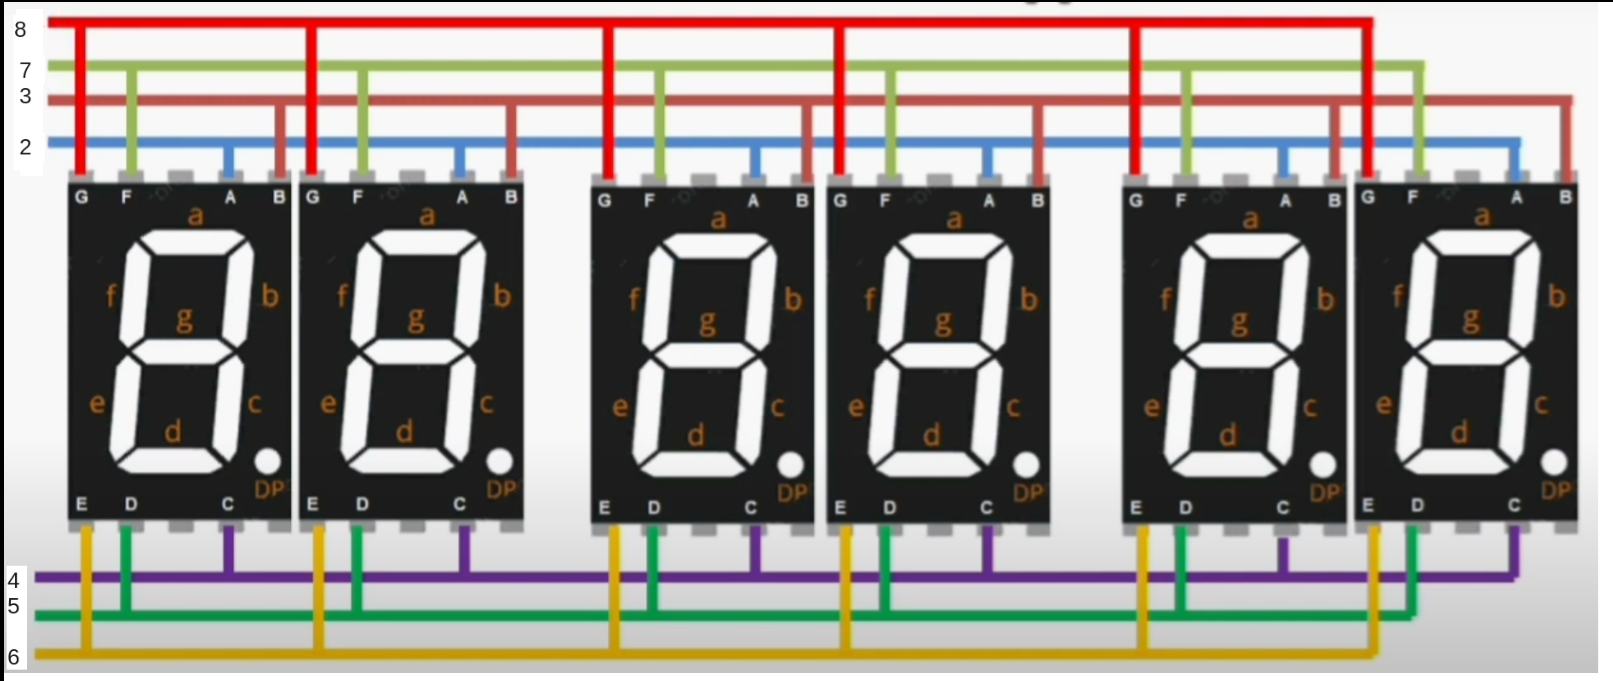
\includegraphics[width=0.75\columnwidth]{Connections/Connections.png}
\end{center}

The pins of seven segment display, Namely, a,b,c,d,e,f,g, are connected together.These are then connected to 2,3,4,5,6,7,8 pins on the arduino.\\
The pin between a and f is COM(Common pin) of first display is connected to pin 9 on arduino.Similarly 2nd,3rd,4th,5th,6th COM pins are connected to 10,11,12,13,A0 pins on the arduino.\\
The must be a resistor of \SI{220}{\ohm} between the COM pin and arduino pins to avoid high voltage which may  burn out the segments, making them dim permanently or stop working entirely.\\
The dot pins are grounded.\\

\section{Working Principle}

\subsection{Multiplexing}
\begin{enumerate}
    \item Multiplexing is a technique used to control multiple seven-segment displays using fewer Arduino pins by turning on one display at a time very quickly.
    \item This creates an illusion that all displays are ON simultaneously.
    \item All A-G segment pins of the displays are connected together and controlled by the same Arduino pins.
    \item The Arduino activates one display, sends the digit data, then quickly switches to the next display.
    \item The Arduino rapidly cycles through each display thousands of times per second, making it appear that all are ON at the same time.
\end{enumerate}

\subsection{Software implementation}
The following code is used to program the Arduino for controlling the digital clock. It handles multiplexing of six seven-segment displays, updates the time, and manages display refreshing.\\

\begin{lstlisting}[language=C++]


#include "Arduino.h"

#define PINS_COUNT 6 // Number of common anode control pins (for each display)
#define NO_SEGMENTS 7 // Number of segments per display (a to g)

// Defining control pins for each seven-segment display
int pins[PINS_COUNT] = {9, 10, 11, 12, 13, A0};

// Defining segment control pins (a to g)
int segPins[NO_SEGMENTS]={2,3,4,5,6,7,8};

void setup() {
	 for (int i = 0; i < 7; i++) {
    pinMode(segPins[i], OUTPUT);
  }

    for (int i = 0; i < PINS_COUNT; i++) {
        pinMode(pins[i], OUTPUT);
    }
}
void sevenseg(int a,int b, int c ,int d,int e ,int f,int g)
{
	digitalWrite(2,a);
	digitalWrite(3,b);
	digitalWrite(4,c);
	digitalWrite(5,d);
	digitalWrite(6,e);
	digitalWrite(7,f);
	digitalWrite(8,g);
}
// Function to display a digit (0-9) on the seven-segment display

void displayDigit(int digit) {
	switch(digit){
		case 0:sevenseg(0, 0, 0, 0, 0, 0, 1);break;
		case 1:sevenseg(1, 0, 0, 1, 1, 1, 1);break;
		case 2:sevenseg(0, 0, 1, 0, 0, 1, 0);break;
		case 3:sevenseg(0, 0, 0, 0, 1, 1, 0);break;
		case 4:sevenseg(1, 0, 0, 1, 1, 0, 0);break;
		case 5:sevenseg(0, 1, 0, 0, 1, 0, 0);break;
		case 6:sevenseg(0, 1, 0, 0, 0, 0, 0);break;
		case 7:sevenseg(0, 0, 0, 1, 1, 1, 1);break;
		case 8:sevenseg(0, 0, 0, 0, 0, 0, 0);break;
		case 9:sevenseg(0, 0, 0, 0, 1, 0, 0);break;		
}
}
void loop() {
    //Extracting individual digits for each display
    int h1 = 0;  // Tens place of hours
    int h2 = 0;  // Units place of hours
    int m1 = 0;  // Tens place of minutes
    int m2 = 0;  // Units place of minutes
    int s1 = 0;  // Tens place of seconds
    int s2 = -1;  // Units place of seconds
do{
//Loop to display time for 24 hours
for(int i=0;i<82;i++){

    // Multiplexing for six displays
    digitalWrite(pins[0], HIGH);
    displayDigit(h1);
    delay(2);
    
    digitalWrite(pins[0], LOW);
    digitalWrite(pins[1], HIGH);
    displayDigit(h2);
    delay(2);
    
    digitalWrite(pins[1], LOW);
    digitalWrite(pins[2], HIGH);
    displayDigit(m1);
    delay(2);
    
    digitalWrite(pins[2], LOW);
    digitalWrite(pins[3], HIGH);
    displayDigit(m2);
    delay(2);
    
    digitalWrite(pins[3], LOW);
    digitalWrite(pins[4], HIGH);
    displayDigit(s1);
    delay(2);
    
    digitalWrite(pins[4], LOW);
    digitalWrite(pins[5], HIGH);
    displayDigit(s2);
    delay(2);
    
    digitalWrite(pins[5], LOW);
}
//Modifying Display after each second.
    s2++;
    if(s2>=10){
	    s2=0;
	    s1++;
    }
    if(s1>=6){
	    s1=0;
	    m2++;
    }
    if(m2>=10){
	    m2=0;
	    m1++;
    }
    if(m1>=6){
	    m1=0;
	    h2++;
    }
    if(h2>=10){
	    h2=0;
	    h1++;
    }
    if(h1>=3){
	    h1=0;
    }
    if (h1 == 2 && h2 == 4) {  
    h1 = 0;
    h2 = 0;
}

}while(s2>=0);
}

\end{lstlisting}

\section{Precautions}

\subsection{Hardware}
\begin{enumerate}
    \item  Always connect \SI{220}{\ohm} resistors in series with the seven-segment display segments to prevent excessive current draw and potential damage to the Arduino.
    \item  Double-check wiring to ensure no accidental short circuits, which could damage the microcontroller or display.
    \item  Before making any changes to the circuit, disconnect the Arduino from the power source to prevent accidental damage.
\end{enumerate}

\subsection{Software}
\begin{enumerate}
    \item  Ensure that the delay in the multiplexing loop is optimized to avoid flickering or unreadable digits. A 1.5-5ms delay per digit works well.
    \item Before uploading the code, double-check that the correct pins are assigned to the display segments and common anodes.
\end{enumerate}
\end{document}

